%%
%% This is file `sample-manuscript.tex',
%% generated with the docstrip utility.
%%
%% The original source files were:
%%
%% samples.dtx  (with options: `manuscript')
%% 
%% IMPORTANT NOTICE:
%% 
%% For the copyright see the source file.
%% 
%% Any modified versions of this file must be renamed
%% with new filenames distinct from sample-manuscript.tex.
%% 
%% For distribution of the original source see the terms
%% for copying and modification in the file samples.dtx.
%% 
%% This generated file may be distributed as long as the
%% original source files, as listed above, are part of the
%% same distribution. (The sources need not necessarily be
%% in the same archive or directory.)
%%
%% Commands for TeXCount
%TC:macro \cite [option:text,text]
%TC:macro \citep [option:text,text]
%TC:macro \citet [option:text,text]
%TC:envir table 0 1
%TC:envir table* 0 1
%TC:envir tabular [ignore] word
%TC:envir displaymath 0 word
%TC:envir math 0 word
%TC:envir comment 0 0
%%
%%
%% The first command in your LaTeX source must be the \documentclass command.
%%%% Small single column format, used for CIE, CSUR, DTRAP, JACM, JDIQ, JEA, JERIC, JETC, PACMCGIT, TAAS, TACCESS, TACO, TALG, TALLIP (formerly TALIP), TCPS, TDSCI, TEAC, TECS, TELO, THRI, TIIS, TIOT, TISSEC, TIST, TKDD, TMIS, TOCE, TOCHI, TOCL, TOCS, TOCT, TODAES, TODS, TOIS, TOIT, TOMACS, TOMM (formerly TOMCCAP), TOMPECS, TOMS, TOPC, TOPLAS, TOPS, TOS, TOSEM, TOSN, TQC, TRETS, TSAS, TSC, TSLP, TWEB.
% \documentclass[acmsmall]{acmart}

%%%% Large single column format, used for IMWUT, JOCCH, PACMPL, POMACS, TAP, PACMHCI
% \documentclass[acmlarge,screen]{acmart}

%%%% Large double column format, used for TOG
% \documentclass[acmtog, authorversion]{acmart}

%%%% Generic manuscript mode, required for submission
%%%% and peer review
\documentclass[sigconf,screen,review]{acmart}
%% Fonts used in the template cannot be substituted; margin 
%% adjustments are not allowed.
%%
%% \BibTeX command to typeset BibTeX logo in the docs
\AtBeginDocument{%
  \providecommand\BibTeX{{%
    \normalfont B\kern-0.5em{\scshape i\kern-0.25em b}\kern-0.8em\TeX}}}

%% Rights management information.  This information is sent to you
%% when you complete the rights form.  These commands have SAMPLE
%% values in them; it is your responsibility as an author to replace
%% the commands and values with those provided to you when you
%% complete the rights form.
\setcopyright{acmcopyright}
\copyrightyear{2023}
\acmYear{2023}
\acmDOI{XXXXXXX.XXXXXXX}

%% These commands are for a PROCEEDINGS abstract or paper.
\acmConference[Conf '23]{
  %International Symposium on Spatial and Temporal Data
}{
  %August 23--25, 2023
}{
  %Calgary, Canada
}
%
%  Uncomment \acmBooktitle if th title of the proceedings is different
%  from ``Proceedings of ...''!
%
\acmBooktitle{
%SSTD '23: International Symposium on Spatial and Temporal Data, August 23--25, 2023, Calgary, Canada}
\acmPrice{15.00}
\acmISBN{978-1-4503-XXXX-X/18/06}


%%
%% Submission ID.
%% Use this when submitting an article to a sponsored event. You'll
%% receive a unique submission ID from the organizers
%% of the event, and this ID should be used as the parameter to this command.
%%\acmSubmissionID{123-A56-BU3}

%%
%% end of the preamble, start of the body of the document source.

%\usepackage{titlesec}
%\titlespacing*{\section}{5pt}{0.1\baselineskip}{0.2\baselineskip}

\usepackage{subcaption}
%% For algorithms...
\usepackage{algorithm}
\usepackage{algpseudocode}
\algnewcommand\algorithmicforeach{\textbf{for each}}
\algdef{S}[FOR]{ForEach}[1]{\algorithmicforeach\ #1\ \algorithmicdo}
\algnewcommand\algorithmicswitch{\textbf{switch}}
\algnewcommand\algorithmiccase{\textbf{case}}
\algdef{SE}[SWITCH]{Switch}{EndSwitch}[1]{\algorithmicswitch\ #1\ \algorithmicdo}{\algorithmicend\ \algorithmicswitch}
\algdef{SE}[CASE]{Case}{EndCase}[1]{\algorithmiccase\ #1}{\algorithmicend\ \algorithmiccase}
\algtext*{EndSwitch}
\algtext*{EndCase}

\setlength{\textfloatsep}{2pt plus 1.0pt minus 2.0pt}

\usepackage{tikz}
\usetikzlibrary{shapes, arrows}

\begin{document}

%%
%% The "title" command has an optional parameter,
%% allowing the author to define a "short title" to be used in page headers.
\title{Parallel finding of moving flock patterns}

%%
%% The "author" command and its associated commands are used to define
%% the authors and their affiliations.
%% Of note is the shared affiliation of the first two authors, and the
%% "authornote" and "authornotemark" commands
%% used to denote shared contribution to the research.

\author{Andres Calderon-Romero}
%\authornote{All authors contributed equally to this research.}
\email{acald013@ucr.edu}
\affiliation{
  \institution{University of California, Riverside}
  \country{}
  \city{}
}

\author{Petko Balakov}
\email{petko@}
\affiliation{
  \institution{Esri}
  \country{}
  \city{}
}

\author{Marcos Vieira}
\email{marcos@}
\affiliation{
  \institution{Google}
  \country{}
  \city{}
}

\author{Vassilis J. Tsotras}
\email{tsotras@cs.ucr.edu}
\affiliation{
  \institution{University of California, Riverside}
  \country{}
  \city{}
}

%%
%% By default, the full list of authors will be used in the page
%% headers. Often, this list is too long, and will overlap
%% other information printed in the page headers. This command allows
%% the author to define a more concise list
%% of authors' names for this purpose.
\renewcommand{\shortauthors}{Calderon, et al.}

%%
%% The abstract is a short summary of the work to be presented in the
%% article.
\begin{abstract}

\end{abstract}

%%
%% The code below is generated by the tool at http://dl.acm.org/ccs.cfm.
%% Please copy and paste the code instead of the example below.
%%
\begin{CCSXML}
<ccs2012>
   <concept>
       <concept_id>10010147.10010169.10010170</concept_id>
       <concept_desc>Computing methodologies~Parallel algorithms</concept_desc>
       <concept_significance>500</concept_significance>
       </concept>
   <concept>
       <concept_id>10002951.10002952.10002971</concept_id>
       <concept_desc>Information systems~Data structures</concept_desc>
       <concept_significance>500</concept_significance>
       </concept>
   <concept>
       <concept_id>10010147.10010919.10010172.10003817</concept_id>
       <concept_desc>Computing methodologies~MapReduce algorithms</concept_desc>
       <concept_significance>500</concept_significance>
       </concept>
 </ccs2012>
\end{CCSXML}

\ccsdesc[500]{Computing methodologies~Parallel algorithms}
\ccsdesc[500]{Information systems~Data structures}
\ccsdesc[500]{Computing methodologies~MapReduce algorithms}

%%
%% Keywords. The author(s) should pick words that accurately describe
%% the work being presented. Separate the keywords with commas.
\keywords{Mobile patterns}

%%\received{20 February 2007}
%%\received[revised]{12 March 2009}
%%\received[accepted]{5 June 2009}

%%
%% This command processes the author and affiliation and title
%% information and builds the first part of the formatted document.
\maketitle

\section{Introduction}
Technology advances in last past decades have triggered an explosion in the capture of spatio-temporal data.  The increase popularity of GPS devices and smart-phones together with the emerging of new disciplines such as the Internet of Things and Satellite/UAS high-resolution imagery have made possible to collect vast amount of data with a spatial and temporal component attached to them.

Together with this, the interest to extract valuable information from such large databases has also appeared.  Spatio-temporal queries about most popular places or frequent events are still useful, but more complex patterns are recently shown an increase of interest.  In particular, those what describe group behaviour of moving objects through significant periods of time.  Moving cluster \cite{kalnis_discovering_2005}, convoys \cite{jeung_discovery_2008}, flocks \cite{gudmundsson_computing_2006} and swarm patterns \cite{li_swarm:_2010} are new movement patterns which unveil how entities move together during a minimum time interval. 

Applications for this kind of information are diverse and interesting, in particular if they come in the way of trajectory datasets \cite{jeung_trajectory_2011, huang_mining_2015}. Case of studies range from transportation system management and urban planning \cite{di_lorenzo_allaboard:_2016} to Ecology \cite{la_sorte_convergence_2016}.  For instance, \cite{turdukulov_visual_2014} explore the finding of complex motion patterns to discover similarities between tropical cyclone paths.  Similarly, \cite{amor_persistence_2016} use eye trajectories to understand which strategies people use during a visual search. Also, \cite{holland_movements_1999} tracks the behavior of tiger sharks in the coasts of Hawaii in order to understand their migration patterns.

In particular, a moving flock pattern show how objects move close enough during a given time period.  Closeness is defined by a disk of a given radius where the entities must keep inside.  Given that the disk can be situated at any location, it is not a trivial problem.  In deed, \cite{gudmundsson_computing_2006} claims that find flock patterns where the same entities stay together during their duration is a NP-hard problem. \cite{vieira_2009} proposed the BFE algorithm which the first approach to be able to detect flock patterns in polynomial time.

Despite the fact that much more data become available, state-of-the-art techniques to mine complex movement patterns still depict poor performance for big spatial data problems.  This work presents a parallel algorithm to discover moving flock patterns in large trajectory databases.  It is thought that new trends in distributed in-memory frameworks for spatial operations could help to speed up the detection of this kind of patterns.

\section{Related work}
Recently increase use of location-aware devices (such as GPS, Smart phones and RFID tags) has allowed the collection of a vast amount of data with a spatial and temporal component linked to them.  Different studies have focused in discovering and analyzing this kind of collections \cite{leung_knowledge_2010, miller_geographic_2001}.  In this area, trajectory datasets have emerged as an interesting field where diverse kind of patterns can be identified \cite{zheng_computing_2011, vieira_spatio-temporal_2013}.  For instance, authors have proposed techniques to discover motion spatial patterns such as moving clusters \cite{kalnis_discovering_2005}, convoys \cite{jeung_discovery_2008} and flocks \cite{benkert_reporting_2008, gudmundsson_computing_2006}.  In particular, \cite{vieira_2009} proposed BFE (Basic Flock Evaluation), a novel algorithm to find moving flock patterns in polynomial time over large spatio-temporal datasets. 

A flock pattern is defined as a group of entities which move together for a defined lapse of time \cite{benkert_reporting_2008}.  Applications to this kind of patterns are rich and diverse.  For example, \cite{calderon_romero_mining_2011} finds moving flock patterns in iceberg trajectories to understand their movement behavior and how they related to changes in ocean's currents. 

The BFE algorithm presents an initial strategy in order to detect flock patterns.  In that, first it finds disks with a predefined diameter ($\varepsilon$) where moving entities could be close enough at a given time interval.  This is a costly operation due to the large number of points and intervals to be analyzed ($\mathcal{O}(2n^2)$ per time interval).  The technique uses a grid-based index and a stencil to speed up the process, but the complexity is still high.

\cite{calderon_romero_mining_2011} and \cite{turdukulov_visual_2014} use a frequent pattern mining approach to improve performance during the combination of disks between time intervals.  Similarly, \cite{tanaka_improved_2016} introduce the use of plane sweeping along with binary signatures and inverted indexes to speedup the same process.  However, the above-mentioned methods still keep the same strategy as BFE to find the disks at each interval.  

\cite{arimura_finding_2014} and \cite{geng_enumeration_2014} use depth-first algorithms to analyze the time intervals of each trajectory to report maximal duration flocks.  However, these techniques are not suitable to find patterns in an on-line fashion.

Given the high complexity of the task, it should not be surprising the use of parallelism to increase performance.  \cite{fort_parallel_2014} use extreme and intersection sets to report maximal, longest and largest flocks on the GPU with the limitations of its memory model.  

Indeed, despite the popularity of cluster computing frameworks (in particular whose supporting spatial capabilities \cite{eldawy_spatialhadoop:_2014, yu_demonstration_2016, pellechia_geomesa:_2015-1, xie_simba:_2016-1}) there are not significant advances in this area.  At the best of our knowledge, this work is the first to explore in-memory distributed systems towards the detection of moving flock patterns.



\section{Methods}
%\IEEEPARstart{T}{his} 
This section explains two alternative methodologies to find moving flock patterns in large spatio-temporal datasets using modern distributed frameworks to divide and parallelize the workload.  Before to explain the details of our contributions we will explains the in a general manner the details of the current state-of-the-art to highlight the challenges and drawbacks at the moment to dealt with very large spatio-temporal datasets.

\subsection{The BFE algorithm}
The alternatives we will discuss later follows closely the steps explained at \cite{vieira_2009}.  In this work, the authors proposed the Basic Flock Evaluation (BFE) algorithm to find flock patterns on trajectory databases.  The details of the algorithm can be accessed at the source but we will explain the main aspects in a general view.  It is important to clarify that BFE runs in two phases: firstly, it finds valid disks in the current time instant; secondly, it combines previous flocks with the recently discovered disks to extend them and report them.  

The main inputs of the BFE algorithm are a set of points, a minimum distance $\varepsilon$ which will define the diameter of the disks where the moving entities should lay, a minimum number of entities $\mu$ at each disk and a minimum duration $\delta$ which is the minimum number of time units the entities should be keep together to be considered a flock.  Based on these inputs,  figure \ref{fig:MF_flowchart} breaks down schematically the work flow  of this phase where we can identify 4 general steps.  The main goal of this phase is to find a set of valid disks at each time instant to allow further combinations with subsequent sets of disks coming in the future.

\begin{figure}
    \centering
    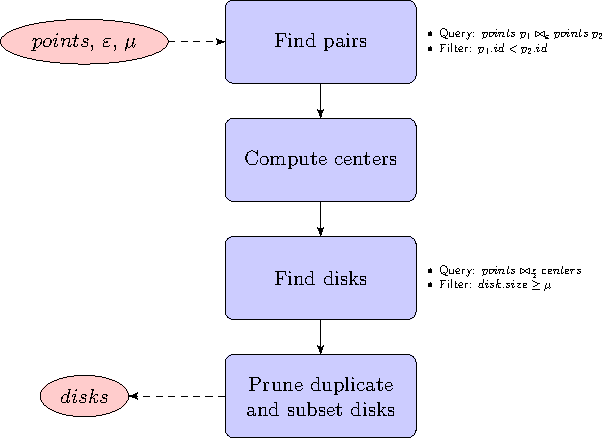
\includegraphics[width=\linewidth]{figures/MF_flowchart}
    \caption{General steps in phase 1 of the BFE algorithm.}\label{fig:MF_flowchart}
\end{figure}

The main steps in phase one can are explained as follows:
\begin{enumerate}
    \item Pair finding:  Using the $\varepsilon$ parameter, the algorithm query the set of points to get the set of pairs which laid at a maximum distance of $\varepsilon$ units.  Usually, it is a distance self-join operation over the set of points using $\varepsilon$ as the distance parameter.  The query also pays attention to do not return pair duplicates.  For instance, the pair between point $p_1$ and $p_2$ is the same that pair between $p_2$ and $p_1$ and just one of them should be reported (the id of each point is used to filter duplicates).
    \item Center computation:  From the previous set of pairs, each tuple is the input of a simple computation to locate the centers of the two circles of radius $\frac{\varepsilon}{2}$ which circumference laid on the input points.  The pseudocode of the procedure can be seen in appendix \ref{app:centers}.
    \item Disk finding: Once the centers have been identified, a query to collect the points around those centers is needed in order to group the set of points which laid $\varepsilon$ distance units each other.  This is done by running a distance join query between the set of points and the set of centers using $\frac{\varepsilon}{2}$ as the distance parameter. Therefore, a disk will be defined by its center and the IDs of the points around it. At this stage, a filter is applied to remove those disks which collect less than $\mu$ entities around it.
    \item Disk pruning: It is possible than a disk collects the same set of points, or a subset, of the set of points of another disk.  In such cases the algorithm should report just that one which contains the others.  An explanation of the procedure can be seen in appendix \ref{app:disks}.
\end{enumerate}

It is important to note that BFE also proposes a grid index structure in this phase to speed up spatial operations.  The algorithm divides the space area in a grid of $\varepsilon$ side (see figure \ref{fig:grid} from \cite{vieira_2009}).  In this way, BFE just processes each grid and its 8 neighbor grids.  It does not need to query grids outside of its neighborhood given that points in other grids are far away to affect the results.

\begin{figure}
    \centering
    \includegraphics[clip,trim=13cm 21.75cm 4.1cm 1.85cm]{figures/grid}
    \caption{The grid-based index structure proposed at \cite{vieira_2009}.}\label{fig:grid}
\end{figure}

The second phase is more straightforward.  Figure \ref{fig:FF_flowchart} explains schematically what is done once the set of current disks (as explained in figure \ref{fig:MF_flowchart}) is found at every time instant.  This phase performs a recursion using the current set of disks and the previous set of flocks which comes from the  previous time instant.  Due to we do not know where and how far a group of entities can move in the next time instant, a cross product between both sets is required.  

\begin{figure}
    \centering
    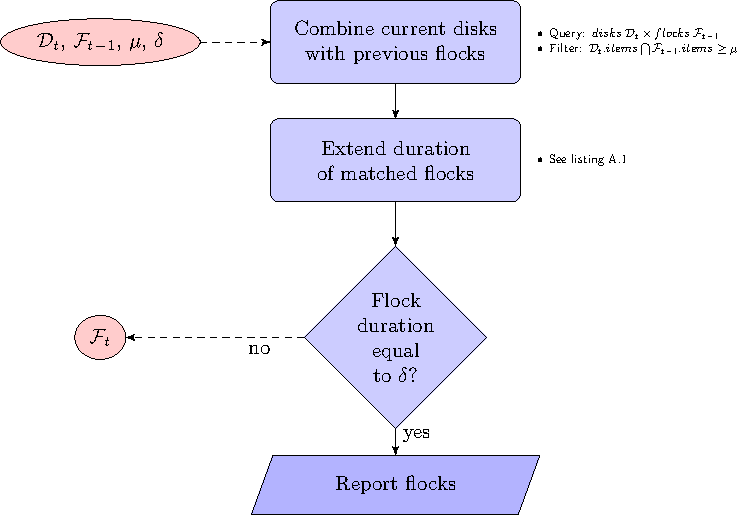
\includegraphics[width=\linewidth]{figures/FF_flowchart}
    \caption{Steps in BFE phase two. Combination, extension and reporting of flocks.}\label{fig:FF_flowchart}
\end{figure}

However, just disks which match the entities of previous flocks are kept.  Indeed, only when the size of common items is greater than $\mu$ we keep the pair.  Then, it updates the end time and duration of the filtered flocks.  This information is used to decide if it is time to report a flock or keep it for further analysis.  If the duration has reached the minimum duration $\delta$, a flock is reported and removed from the set.  The remaining flocks are sent to the next iteration for further evaluation in the next time instant.

Similarly, figure \ref{fig:FF_stages} illustrates the recursion and how the set of flocks from previous time instants feeds the next iteration.  The example assumes a $\delta$ value of 3, so it starts reporting flock since time instant $t_2$.  Note that time instants $t_0$ and $t_1$ are initial conditions.  At the very beginning of the execution, we just can find valid disks at $t_0$ which immediately are transformed to flocks of duration 1 and feed the next time instant.  At $t_1$ we can find a new set of disks $\mathcal{D}_1$ which combines with the set of previous flocks $\mathcal{F}_0$.  It updates the information of each flock accordingly but it does not report any flock yet.  From now on, subsequent time instants follows strictly the steps summarized on figure \ref{fig:FF_flowchart}.

\begin{figure}[!ht]
    \centering
    \includegraphics[width=\linewidth]{figures/FF_stages}
    \caption{BFE phase 2 example explaining the recursion of the set of flocks along time instants and the initial conditions.}\label{fig:FF_stages}
\end{figure}

\subsection{Bottlenecks in BFE and possible solutions}
There are some steps during the execution of BFE which are particularly affected when it deals with very large datasets.  Firstly, we will focus on phase 1 of BFE.  In figure \ref{fig:example}, the steps of this phase are illustrated for a sample dataset.  You can see that the number of centers and disks found is considerable large in comparison with the final set of valid disks.  Indeed, the finding of centers and the following operations grows quadratic depending on the number of points and possible pairs (which itself depend on the $\varepsilon$ parameter).   

\cite{vieira_2009} claims that the number of centers, and consequent disks, to be evaluated is equal to $2\lvert\tau\rvert^2$ where $\tau$ is the number of trajectories.  However, our experience show that there are a large number of duplicate and subset disks which are later pruned in the final stage.  This behaviour is exacerbated no just in very large datasets but also in those with areas with high density of moving entities.

\begin{figure*}
    \centering
    \includegraphics[width=\linewidth]{figures/MF_stages/flow}
    \caption{Example of BFE execution on a sample dataset.}\label{fig:example}
\end{figure*}

As solution for this issue, we proposed a partition strategy to divide the study area in smaller sections which can be evaluated in parallel.  The strategy has three steps: first, a partition and replication stage, then the flock discovery in each local partition and finally the merge stage where we collect and unify the results.  Let's explain each stage in more detail:

\begin{itemize}

\item Partition and Replication: Figure \ref{fig:partrep} shows a brief example of the partition and replication stage.  Note that it is possible to use different types of spatial indexes (grids, r-tree, quadtree, etc.) to create spatial partitions over the input dataset.  In the case of the example we use a quadtree which creates 7 partitions.  Now, we need to ensure that each partition has access to all the required data to complete the finding of flocks locally.  To accomplish this, all the points laying at $\varepsilon$ distance of the border of its partition are replicated to adjacent partitions.  At the right of figure \ref{fig:partrep},  it can be seen each partition surrounded by a dotted area with the points which need to be copied from its neighbor partitions.  At this point, each partition is ready to be submitted to different nodes for local processing.

\begin{figure}
    \centering
    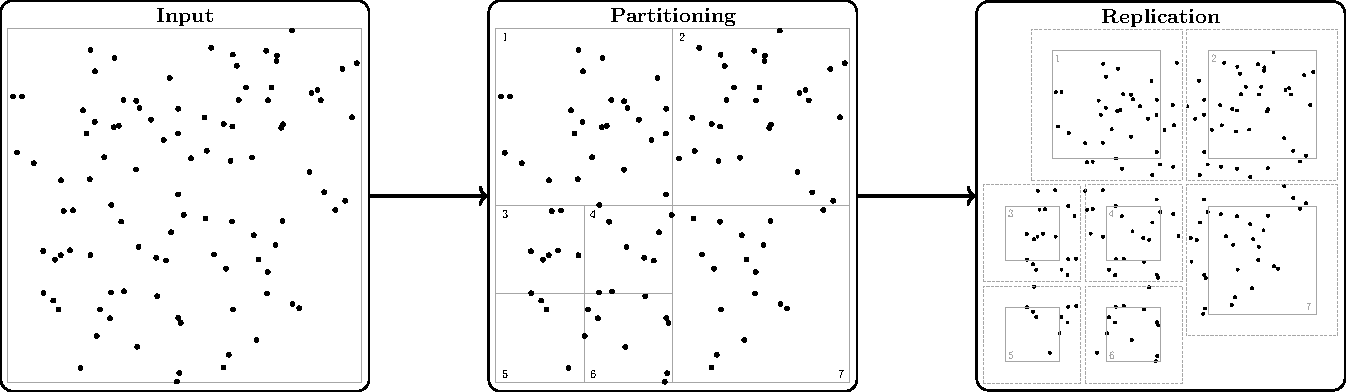
\includegraphics[width=\linewidth]{figures/MF_stages/P123}
    \caption{An example of partitioning and replication on a sample dataset.}\label{fig:partrep}
\end{figure}

\item Local discovery: Once we have all the data we need at each partition we can run the steps of the phase 1 of the BFE algorithm locally (as were explained on figure \ref{fig:MF_flowchart}).  Actually, you can see that the example of figure \ref{fig:example} describes the execution using the partition 2's points of figure \ref{fig:partrep} as sample data.

\item Merging:  In order to merge back the results we will have to pay special attention to disks laying close to the border of each partition.  We will show that if the position of disk centers lay inside of the current partition they will be safe to operate but those located in the expansion zone or outside of it will require to be treated to avoid duplicate reports.  

Disks with centers in the expansion zone will be repeated in contiguous partitions and, therefore, they will lead to duplication.  In addition, it is possible that pairs of points generates disks with centers outside of the expansion zone.  For example, Fig. \ref{subfig:mergeA} illustrates the case.  Disks $a^\prime$ and $b^\prime$ are generated for points in partitions 1 and 2 respectively, however both are located outside of their expansion zone boundaries and we should to avoid to report them twice.  We present lemma \ref{lemma:disks} to show that we can safely remove those kind of disks.

\begin{lemma}\label{lemma:disks}
A disk with its center laying in the expansion zone or outside of it can be discarded as they will be correctly evaluated by one of the partitions in its neighborhood. 
\end{lemma}

\begin{proof}
  In order to support our proof we will define some concepts:  First, we will divide the area of a partition in three zones to clarify our assumptions:  we already talked about the \textit{expansion zone} as the area beyond the border of a partition (between black line and dotted red line in figure \ref{subfig:mergeA}) and a width equal to $\varepsilon$.  The \textit{border zone} is a strip of width equal to $\varepsilon$ touching the interior border of a partition.  In figure \ref{subfig:mergeA}, it is compromised by the dotted blue and the black lines.  The \textit{safe zone} will be the remaining internal area in the partition which is not covered by the border zone.  Second, we will call the contiguous partition which replicate a particular disk with the current one as the \textit{replicated partition}. In figure \ref{subfig:mergeA}, the partition 2 is the replicated partition of partition 1 and vice versa.

  From here, it will be clear that there is a symmetric relation between the disks in the border and expansion zones in the current partition and the disks in its replicated partition.  We can certainly said that if a disk is located in the border zone of the current partition, it will be located in the expansion zone of its replicated partition.  Similarly, any disk with a center laying outside of the expansion zone of the current partition will be located in the safe zone of its replicated partition.  Keeping just the disks with centers laying in the current partition (border or safe zone) will be enough to ensure no lost of information (Fig. \ref{subfig:mergeB}).
\end{proof}

\begin{figure*}
    \centering
    \subfloat[\label{subfig:mergeA}]{%
        \includegraphics[width=0.48\linewidth, page=3]{figures/merge}
    }
    \hfill
    \subfloat[\label{subfig:mergeB}]{%
        \includegraphics[width=0.48\linewidth, page=4]{figures/merge}
    }
    \caption{Merging strategy.}\label{fig:merge}
\end{figure*}

\subsection{Additional improvements during local execution}
Even the partition strategy could reduce the size of the points to be processed at each local partition , it is possible to introduce some filter techniques which allows to reduce the impact in the creation of centers and disks and subsequent pruning.  This section explains the use of maximal cliques and minimum bounding circles (MBC) techniques as heuristics to improve the finding of disk at local level.

In graph theory, a clique is a subset of vertices forming a subgraph where all of their nodes share connections among them.  It is said that the induced subgraph is complete.  Similarly, a maximal clique happens when no additional vertex can be included in the current clique, that is, there is not a superset of vertices which could include the current clique \cite{bron_algorithm_1973}.  Although it is know that finding all maximal cliques is a problem of high complexity, studies claims that working on relatively small real-worlds graphs, they can be found in near-optimal time \cite{eppstein_listing_2010}.

Now, in our approach, it can be noted that after obtaining the set of pairs at the beginning of the BFE algorithm, we can see the result as a graph where the points are the vertices and the connections between nearby points are the edges.  So it is possible to run an algorithm (i.e. Bron-Kerbosch) over that graph to get a set of maximal cliques.

The advantage to find a set of cliques is that we will have access to set of points inside of each clique that by sure must generate one or more disks.  Given the condition of the maximal cliques, all the points inside them are $\varepsilon$ distance each other, and we can know that no other point must be included because that contradicts the definition of a maximal clique.  That constitutes a kind of sub-partitioning technique where we could do additional processing. For example, a simple filter we can apply is to remove those cliques which number of points are less than the $mu$ parameter given that those cliques will be unable to generate disks that fulfill that condition.

To introduce the next filter we need define the concept of minimum bounding circle (MBC).  Algorithms for MBC finding aims to return the center and minimum radius possible of a circle that encloses all the items of a set of points in the plane.  One of the most representative algorithm is proposed at \cite{welzl_mbc_1991} which is able to solve the problem in linear time.

The intention to use MBC algorithms at this stage is to detect maximal cliques where all their points can be enclosed in one single disk.  If that is the case, we could report directly the MBC result and save the costly computation of finding centers and pruning duplicates.  This can bring important improvements especially in datasets where the density of points is high. 

However, we have to clarify that when an unique MBC to cover all the points is not possible, the traditional steps (BFE algorithm) should be applied over them.  Finally, disks from both branches are unified and a final pruning is done to remove possible duplication.  This final step should not be costly because most of the pruning is done at maximal clique level.

Figure \ref{fig:CMBC_flowchart} shows a schematic flow chart of the steps for this alternative.

\begin{figure}
    \centering
    \includegraphics[width=\linewidth]{figures/CMBC_flowchart}
    \caption{Flow chart for the maximal clique and MBC filters.}\label{fig:CMBC_flowchart}
\end{figure}

\end{itemize}


%%
%% The acknowledgments section is defined using the "acks" environment
%% (and NOT an unnumbered section). This ensures the proper
%% identification of the section in the article metadata, and the
%% consistent spelling of the heading.
%\begin{acks}
%\end{acks}

%%
%% The next two lines define the bibliography style to be used, and
%% the bibliography file.
\balance
\bibliographystyle{ACM-Reference-Format}
\bibliography{pflocks}

\end{document}
